\chapter{IRK: Puntu-Finkoa.}

\section{Sarrera.}

Gure helburua, biribiltze errore txikia duen IRK metodoaren inplementazioa proposatzea da. Integrazioaren exekuzio denborak onargarriak izan daitezen behartuta, honako aurrebaldintza finkatu dugu: ekuazio diferentzialaren eskuin aldeko funtzioaren 
sarrera eta irteera argumentuak makina zenbakiak izatea, hau da, konputagailuan Hardware bidezko exekuzioa (azkarra) duen koma-higikorrezko aritmetika erabiltzea. Gaur-egun, zientzia-konputazioan \it{double} ($64$ bit) koma-higikorrezko aritmetikarekin lan egiten da eta beraz, praktikan erabiltzaileak ekuazio diferentziala \it{double} datu-mota honetan zehaztuko duela suposatuko dugu.      

\paragraph*{} Lehenengo Hairer-en inplementazioa aztertuko dugu. Ondoren, IRK inplementazioa hobetzeko gure proposamenak azalduko ditugu. Azkenik, zenbakizko gure inplementazioaren emaitzak erakutsiko dugu.

\section{Hairer-en inplementazioa.}

Gure abiapuntua, Haierek \cite{Hairer2008} proposatutako inplementazio hartu dugu.  
Lan honetan, IRK metodo sinplektikoaren puntu-finkoaren inplementazio estandarraren biribiltze errorearen garapen okerraz jabetu ziren eta gainera, metodo sinplektiko esplizituetan agertzen ez zena. Hauen ustez, bi ziren errore honen jatorriak:

\begin{enumerate}
\item Integrazioan $a_{ij}, b_i \in \mathbb{R}$ koefiziente zehatzak erabili ordez, biribildutako $\tilde a_{ij},\tilde b_i \in \mathbb{F}$ erabiltzeak, aplikatutako IRK metodoa zehazki sinpletikoa ez izatea eragiten du.
\item Puntu-finkoaren geratze irizpide estandarra dela eta, urrats bakoitzean errore sistematikoa gertatzen da.
\end{enumerate}    

\paragraph*{}Arrazoi hauek aztertu ondoren, honako konponbideak proposatu zituzten:

\begin{enumerate}
\item Doitasun handiagoko koefizienteak erabili, hauetako bakoitza bi koma-higikorreko koefizienteen batura kontsideratuz $a_{ij}= a^{\ast}_{ij}+\tilde a_{ij}, \ b_i= b^{\ast}_i+\tilde b_i$.
\item Iterazioak geratu, definitutako norma txikitzeari uzten dionean.

\[\triangle ^{[k]} = \max_{i=1,\dots,s}\|Y_i^{[k]}-Y_i^{[k-1]}\|_{\infty} \]
\begin{equation*}
\triangle^{[k]} = 0 \ \ or \  \triangle^{[k]} \geqslant \triangle^{[k-1]}
\end{equation*}
  	 	
\end{enumerate}

Jarraian Hairer-en algoritmoa laburtuko dugu  (notazioa sinplifikatze aldera $Y_{n,i}$ gaiaren ordez, $Y_i$ adierazpena erabiliko dugu).

\begin{algorithm}[h]
 \BlankLine
  $e=0$\;
  \For{$n\leftarrow 1$ \KwTo $endstep$}
  {
   \BlankLine
   $k=0$\;
   Hasieratu  $Y_{i}^{[0]}$\; 
   \BlankLine
   \While{ ($\triangle^{[k]} \ != 0 \ \ and \  \triangle^{[k]} < \triangle^{[k-1]}) $}
   {
    \BlankLine 
    $k=k+1$\;
    $F_{i}^{[k]}=f(Y_{i}^{[k-1]}) $\;
    $Y_{i}^{[k]}=y_{n-1}+ h \ \big(\sum\limits_{j=1}^{s} a^{\ast}_{ij} F_{j}^{[k]} \big) 
                          + h \ \big(\sum\limits_{j=1}^{s} \tilde a_{ij} F_{j}^{[k]} \big)$\; 
    $\triangle ^{[k]} = \max_{i=1,\dots,s}\|Y_{i}^{[k]}-Y_{i}^{[k-1]}\|_{\infty}$\;
   }
   \BlankLine
    $\delta_{n}= \bigg(h \ \big(\sum\limits_{i=1}^{s} b^{\ast}_i F_{i}^{[k]} \big)
               + h \ \big(\sum\limits_{i=1}^{s} \tilde b_i F_{i}^{[k]} \big) \bigg)+e $\;
%    $\delta e=\delta_{n}+e $\;
    $y_n=y_{n-1}+\delta_n$\;
    $e=(y_{n-1}-y_n)+\delta_n$\;            
   \BlankLine
 }
 \caption{Main Algorithm}
\end{algorithm}


\section{Gure inplementazioa.}

IRK metodoaren puntu-finkoaren inplementazioan lau proposamen berri egin ditugu. Lehen bi proposamenak  Hairer-ek bere lanean proposatutako konponbideen hobekuntzak dira. Batetik, IRK-ren birformulazio bat erabiliz, IRK metodoaren koma-higikorrezko koefizienteak sinplektizidade baldintza zehazki betetzea lortuko dugu. Bestetik, geratze irizpidean arazo batzuk topatu ditugu eta arazo hauek gainditzen dituen geratze irizpide sendoagoa garatu dugu. Beste bi proposamenak dagokionez, bata batura-konpensatuari erlazionatuta dago eta bestea biribiltze errorea monitorizatzeko proposamena da.
\paragraph*{} Bestalde kapitulu honen bukaeran, batetik interpolazio bidezko atalen hasieraketa eta bestetik, Gauss-Seidel moduko puntu-finkoaren iterazioak azaldu ditugu. Bukatzeko, gure algoritmoa azalduko dugu.  

\subsection{Koefizienteak (1.proposamena).}

IRK metodoa definitzen duten $a_{ij},b_i$ koefizienteak, biribildutako $\tilde a_{ij},\tilde b_i \in \mathbb{F}$ ordezkatzerakoan, sinpletizide baldintza ez da beteko,
\begin{equation} \label{eq:61}
b_{i}a_{ij}+b_{j}a_{ji}-b_{i}b_{j}=0, \ \ 1 \leqslant i,j \leqslant s.
\end{equation}  
  
Arazo hau gainditzeko asmoarekin, IRK metodoa era honetan birformulatuko dugu,

\begin{equation}
\label{eq:62}
Y_{n,i}=y_n+ \sum\limits_{j=1}^{s} \mu_{ij} L_{n,j},  \ \ L_{n,i}=hb_if(Y_{n,i})
\end{equation}

\begin{equation}
\label{eq:63}
y_{n+1}=y_n+\sum\limits_{i=1}^{s} L_{n,i}
\end{equation}

non 

\begin{equation*}
\mu_{ij}=\frac{a_{ij}}{b_j}, \ \ 1 \le i,j \le s.
\end{equation*}

Eta sinplekzidade baldintza modu honetan berridatziko dugu,

\begin{equation}
\mu_{ij}+\mu_{ji}-1=0, \ \ \ 1 \le i,j \le s.
\end{equation}

\paragraph*{} Formulazio honek  estandarrarekiko duen abantaila handiena , sinplektizidade baldintzan biderketarik agertzen ez denez,  baldintza hau betetzen duten $\tilde \mu_{ij} \in \mathbb{F}$ koefizienteak aurkitzeko bidea errazten zaigu. Zehazki era honetan finkatuko ditugu gure koefizienteak:

\begin{enumerate}
\item $\mu_{ij}$ koefizienteak.\\

Batetik $s$-ataleko Gauss metodoetan, $\tilde \mu_{ii}:=\frac{1}{2}, \ i=1,\dots,s$. Bigarrenik $\tilde \mu_{ij}:=fl(\mu_{ij}), \ 1 \le j < i \le s$ finkatuko dugu. Azkenik $\frac{1}{2} < |\mu_{ij}| <2$ denez, eta Sterbenz-en Teoremaren (ikus. \ref{eq:4311}) arabera  $\tilde \mu_{ji}:=1-\tilde{\mu_{ij}}$ koma-higikorrezko adierazpen zehatza du. Ondorioz, simplektizitate baldintza zehazki betetzen duten koma-higikorrezko $\tilde \mu_{ij}$ koefizienteak lortu ditugu.   

\begin{equation}
\left(\begin{array}{cccc}
    \frac{1}{2}       & 1-fl(\mu_{21}) & \dots & 1-fl(\mu_{s1})      \\
    fl(\mu_{21})      & \frac{1}{2}    & \dots & 1-fl(\mu_{s2})      \\
    \vdots            & \ddots         &       & \vdots              \\
    fl(\mu_{s1})      & fl(\mu_{s2})   & \dots & \frac{1}{2}          \\ 
     \end{array}\right)
\end{equation}

\item $b_{i}$ koefizienteak.\\

Gure inplementazioan, $hbi$ koefizienteak erabiliko ditugu. Batetik, koefiziente hauek simetrikoak direla eta bestetik, $\sum\limits_{i=1}^{s} hb_i=h$ berdintza bete behar dela kontutan hartuz,

\begin{eqnarray}
hb_1=hb_s:= h - \sum\limits_{i=2}^{s-1} hb_i
\end{eqnarray}


\end{enumerate}

\subsection{Geratze irizpidea (2.proposamena).}

Ekuazio inplizituaren (\ref{eq:62}) soluzioaren hurbilpena lortzeko puntu-finkoko iterazioa era honetan definituko dugu. Iterazioaren abiapuntua $Y_i^{[0]}$  finkatu eta $k=1,2,\dots$ iterazioetarako $Y_i^{[k]}$ hurbilpenak lortu dagokigun geratze irizpidea bete arte.

\begin{equation}
L_i^{[k]}=hb_if(Y_i^{[k-1]}), \ \ Y_i^{[k]}=y_n+\sum\limits_{j=1}^{s} \mu_{ij} L_j^{[k]}
\end{equation}
 
\paragraph*{}IRK metodoaren inplementazio estandarrean geratze erizpidea honakoa da,

\begin{equation*}
\triangle^{[k]}=(Y_1^{[k]}-Y_1^{[k-1]},\dots,Y_s^{[k]}-Y_s^{[k-1]}) \in \mathbb{R}^{sd},
\end{equation*}
 
\begin{equation}
\|\triangle^{[k]}\| \le tol
\end{equation}
non $\|.\|$ aurre-finkatutako bektore norma eta \emph{tol} tolerantzia errorea den . Tolerantzia txikiegia aukeratzen bada, gerta daiteke tolerantzia hori ez lortzea eta infinituki iterazioak exekutatzea. Baina tolerantzia ez bada behar adina txikia  aukeratzen, iterazioak puntu-finkora iritsi aurretik geratuko dira eta lortutako $Y_i^{[k]}$ hurbilpenak biribiltze errorea baino errore handiago izango du.

\paragraph*{} Gogoratuz Hairer-ek proposatu zuen geratze irizpidea :  $\triangle^{[k]} = 0$ (puntu-finkora iritsi delako) ;  edo   $\triangle^{[k]} \geqslant \triangle^{[k-1]}$ (biribiltze errorea nagusi delako). Orokorrean, geratze irizpide honek ondo funtzionatzen du baina batzuetan, iterazioak goizegi geratu direla konprobatu dugu. Gure iritziz, honen arrazoia da $\triangle^{[k]} \geqslant \triangle^{[k-1]}$ biribiltze errorea nagusia dela adierazten duen arren, badago $j \in \{1,\dots,sd\}$ osagairik,   $|\triangle_j^{[k]}| < |\triangle_j^{[k-1]}|$ hobetzeko tartea duena. 

\paragraph*{} Gure proposamena azaldutako arazoari soluzioa emateko asmoarekin, iterazioak jarraitzea honako baldintza betetzen ez den bitartean,

\begin{equation}
\exists j \in \{1,\dots,sd\} \ , \ |\triangle_j^{[1]}| >|\triangle_j^{[2]|}>\dots>|\triangle_j^{[k]}|>0.
\end{equation}


\subsection{Batura konpensatua (3.proposamena).}

Integrazioaren zenbakizko soluzioa  $y_n \approx y(t_n)$ ($n=1,2,\dots$) lortzeko, urrats bakoitzean honako batura dugu,
\begin{equation*}
y_n=y_{n-1} + \phi(y_{n-1,h}).
\end{equation*}   

\paragraph*{} IRK metodoetan, $\phi: \mathbb{R}^{[d+1]} \rightarrow \mathbb{R}^d$ gehikuntza,
\begin{equation*}
\phi(y_{n,h})=\sum\limits_{i=1}^{s} L_{n,i},
\end{equation*}

\paragraph*{} non $L_{n,i}$ ($i=1,\dots,s$) inplizituki definitzen diren.

\paragraph*{} Urrats askotako integrazioetan, batura honetan gertatutako biribiltze erroreak doitasun galera garrantzitsua sortzen du. Beraz, zenbakizko integrazioetan biribiltze errorea gutxitzeko oso erabilgarria zaigu batura konpensatu teknika aplikatzea.

\begin{algorithm}[h]
 \BlankLine
  $\tilde {e}_0=0$\;
  \BlankLine
  \For{$n\leftarrow 1$ \KwTo $endstep$}
  {
   $\dots$\;
   \BlankLine
    $\tilde {\delta}_{n}= (\sum\limits_{i=1}^{s} L_{i}^{[k]}) \oplus \tilde {e}_{n-1} $\;
    $\tilde {y}_n=\tilde{y}_{n-1} \oplus \tilde{\delta}_n$\;
    $\tilde {e}_{n}=(\tilde{y}_{n-1} \ominus \tilde{y}_n)\oplus \tilde{\delta}_n$\;            
   \BlankLine
 }
 \caption{Batura konpensatua}
\end{algorithm}

\paragraph*{} $y_n \in \mathbb{R}^{d}$,  $y_n=\tilde y_{n-1}+\tilde \delta_n$ soluzioa zehatza izanik eta $\tilde y_n \in \mathbb{F}^{d}$,  $\tilde y_n=\tilde y_{n-1} \oplus \tilde \delta_n$ koma-higikorreko hurbilpena izanik, lortutako errore estimazioa $\tilde{e_n}$ ,  zehazki benetako biribiltze errorea da,

\begin{equation}
y_n=\tilde {y}_n+\tilde {e}_n. 
\end{equation}

\paragraph*{} Horregatik, IRK metodoaren inplementazioan, inplizituki $Y_{n,i}$ atalak askatzeko ekuazioetan, $\tilde {y}_n$ ordez ($\tilde{y}_n \oplus \tilde{e}_n$) erabiltzea proposatzen dugu,   

\begin{equation}
L_i^{[k]}=hb_if(Y_i^{[k-1]}), \ \ Y_i^{[k]}=\tilde{y}_n \oplus \big(\tilde{e}_n \oplus \sum\limits_{j=1}^{s} \mu_{ij} L_j^{[k]}\big).
\end{equation}

\paragraph{}Aldaketa honekin, lortutako zenbakizko soluzioaren doitasuna pixka bat hobetzea espero dugu. 


\subsection{Biribiltze errorearen estimazioa (4.proposamena).}

Zenbakizko integrazioaren biribiltze errorearen estimazioa, bigarren zenbakizko integrazio baten soluzioaren diferentzia gisa kalkulatuko dugu. Bigarren integrazio honetan, $Y_i^{[k]}$ atalak mantisa txikiagoko zenbakitara biribiltzen ditugu eta horrela doitasun gutxiagoko soluzioa lortzen dugu. 

$r\ge0$ zenbaki osoa, eta $x \in \mathbb{F}$ ($m$ doitasunezko koma-higikorrezko zenbakia) izanik, honako funtzioa definituko dugu,\\

\begin{algorithm}[H]
  \SetAlgoLined\DontPrintSemicolon
  \SetKwFunction{algo}{algo}\SetKwFunction{floatR}{floatR}
  \SetKwProg{myalg}{Algorithm}{}{}
  \SetKwProg{myproc}{Function}{}{}
  \myproc{\floatR {x,r}}{
    $res=(2^r x \oplus x)\ominus 2^r x$\;
    \KwRet res \;}
  \caption{floatR}
\end{algorithm} 

\paragraph*{}Funtzio honek itzultzen duen balioa, $(m-r)$ doitasunezko koma-higikorrezko zenbakia da. Beste modu batera esanda, $m$ biteko koma-higikorrezko $x$ zenbakiaren azken $r$ bitak zeroan jartzen dituen funtzioa.
     
\paragraph*{} $r<m$ zenbaki osoa finkatuta, bigarren integrazioaren puntu-finkoaren iterazioa honela kalkulatuko dugu,

\begin{equation}
L_i^{[k]}=hb_if(Y_i^{[k-1]}), \ \ Y_i^{[k]}=floatR\bigg(\tilde{y}_n \oplus \big(\tilde{e}_n \oplus \sum\limits_{j=1}^{s} \mu_{ij} L_j^{[k]}\big),r\bigg).
\end{equation}

Biribiltze errorearen estimazioa, zenbakizko soluzio nagusiaren $(y^{[main]}_n+e^{[main]}_n)$ eta $r$ balio txiki baterako (adibidez $r=3$) kalkulatutako bigarren zenbakizko soluzioaren $(y^{[sub]}_n+e^{[sub]}_n)$ arteko diferentzia bezala kalkulatuko dugu.  

\begin{equation}
estimazioa_n=(y^{[main]}_n+e^{[main]}_n)-(y^{[sub]}_n+e^{[sub]}_n)
\end{equation}

Gure algoritmoan estimazioa zuzenean lortzeko, bi integrazioak modu eraginkorrean kalkulatzen dira. Urrats bakoitzean, bi integrazioen $Y_i$ ($i=1,\dots,s$) ataletako balioak, biribiltze errorea estimazio handiegia ez den artean,  antzekoak mantentzen dira. Beraz, bigarren integrazioaren iterazio kopuru txikia beharko dugu, lehen integrazioaren bukaerako $Y_i$ ($i=1,\dots,s$) atalen balioak, bigarren integrazioaren $Y_i^{[0]}$ (i = 1, . . . , s) atalen hasieratzeko erabiliz (algoritmoa zehaztu ???).  


\begin{algorithm}[h]
  \BlankLine
  \For{$n\leftarrow 1$ \KwTo $endstep$}
  {
    \BlankLine
    $Y_n^{[0]}=G(Y_{n-1},h)$\;
    $\dots$\;
    $y_{n+1}=y_{n}+\delta_n$\;
    \BlankLine
    \BlankLine
    \eIf{$(initwithfirst)$}
    {$\hat{Y}_{n}^{[0]}=Y_{n}+(\hat{y}_n-y_n)$\;}
    {$\hat{Y}_{n}^{[0]}=G(\hat{Y}_{n-1},,h)$\;}
    $\dots$\;
    $\hat{y}_{n+1}=\hat{y}_{n}+\hat{\delta}_n$\;
    \BlankLine
    \BlankLine
    $estimation_n=(y_n+e_n)-(\hat{y}_n-\hat{e}_n)$\;
    \BlankLine
   }
 \caption{RKG2: errore estimazioa}
\end{algorithm}

\subsection{Atalen hasieraketa.} 

Ideia da, aurreko urratseko uneetako, $(t_{n-1}+hc_i,Y_{n-1,i}), \ i=1,\dots,s$ eta $(t_{n-1}+h,y_{n})$, balioei dagokien polinomio interpolatzailea erabiliz, urrats berriaren atalen hasieraketa  $(t_{n}+hc_i,Y_{n,i}^{[0]}), \ i=1,\dots,s$ kalkulatzea. 

\begin{figure}[h]
\centerline{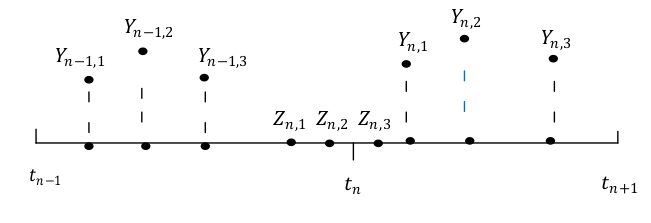
\includegraphics[width=12cm, height=4cm] {Interpolazioa}}
\caption{Interpolazioa.}
\label{fig:bost}
\end{figure}

\paragraph*{}($n-1$) urratseko informazioa erabiliz,
\begin{equation*}
Y_{n-1,i}=y_{n-1}+h \sum\limits_{j=1}^{s} a_{ij} f(Y_{n-1,j})
\end{equation*}

\begin{equation*}
y_n=y_{n-1}+h \sum\limits_{j=1}^{s} b_j f(Y_{n-1,j})
\end{equation*}

\begin{equation}
Y_{n-1,i}=y_n+h \sum\limits_{j=1}^{s} (a_{ij}-b_j) f(Y_{n-1,j})
\end{equation}

\paragraph*{}Dagokion polinomio interpolatzailea,

\begin{equation*}
P(t)=  l_1(t) Y_{n-1,1}+\dots+l_s(t) Y_{n-1,s}+l_{s+1}(t) y_n
\end{equation*}
  
\paragraph*{}non $l_i(t)$ Lagrangiar polinomioa dugu,
\begin{equation*}
 l_i(t)=\prod_{l\neq i,l=1}^{s+1} \frac{(t-(t_{n-1}+hc_l))}{(c_i-c_l)}, \ \ c_{s+1}=1.
\end{equation*}

\paragraph*{}Eta beraz,

\begin{equation}
Y_{n,i} \approx Y_{n,i}^{[0]}= P(t_n+hc_i) = y_n+ h \sum\limits_{j=1}^{s} \lambda_{ij}f(Y_{n-1,j})
\end{equation}

\paragraph*{} Modu honetan s-ataletako IRK metodo bakoitzari dagokion $\lambda_{ij}$ koefiziente interpolatzaileak lortu daitezke. Polinomio interpolatzailearen bidezko hasieraketa ona izango da, emandako urratsa ez bada oso handia eta problema stiff ez denean. Era berean aipatu nahi genuke, atal askotako metodoetan (adibidez $s=16$)  interpolaziozko koefizienteen kalkuluan ezabapen arazoak,  doitasun handian lan egitea behartzen gaituela interpolaziozko hasieraketa ona izateko.  

\subsection{Gauss-Seidel.}

\subsection{Algoritmoa.}

\paragraph*{} Formulazio berriari dagokion algoritmo orokorra,

\begin{algorithm}[H]
 \BlankLine
  $e=0$\;
  \For{$n\leftarrow 1$ \KwTo $endstep$}
  {
   \BlankLine
   Hasieratu  $Y_{i,n}^{[0]} \ \ , \ \ i=1,\dots,s $\;
   \BlankLine
   \While{ (konbergentzia lortu)}
   {
    \BlankLine 
    $L_{n,i}=hb_if(Y_{n,i}) \ \ , \ \  i=1,\dots,s$\;
    $Y_{n,i}=y_{n-1}+ \ \sum\limits_{j=1}^{s} \mu_{ij} L_{n,j}  \ \ , \ \  i=1,\dots,s$\;  
   }
   \BlankLine
    $\delta_{n}= \sum\limits_{i=1}^{s} L_{n,i}+e $\;
    $y_{n}=y_{n-1}+ \delta_{n} $\;
    $e=(y_{n-1}-y_n)+\delta_n$\;
   \BlankLine
 }
 \caption{Main Algorithm}
\end{algorithm}


\paragraph*{} Eta puntu-finkoa erabiliz,

\begin{algorithm}[H]
 \BlankLine
  $e=0$\;
  \For{$n\leftarrow 1$ \KwTo $endstep$}
  {
   \BlankLine
   $k=0$\;
   Hasieratu  $Y_{i}^{[0]}$\;
   \BlankLine
   \While{ (konbergentzia lortu)}
   {
    \BlankLine 
    $k=k+1$\;
    $L_{i}^{[k]}=hb_if(Y_{i}^{[k-1]}) $\;
    $Y_{i}^{[k]}=y_{n-1} + \ \big(e+\sum\limits_{j=1}^{s} \mu_{ij} L_{j}^{[k]}\big)  $\;  
   }
   \BlankLine
    $\delta_{n}= \sum\limits_{i=1}^{s} L_{i}^{[k]}+e $\;
    $y_{n}=y_{n-1}+ \delta_{n} $\;
    $e=(y_{n-1}-y_n)+\delta_n$\;
   \BlankLine
 }
 \caption{Main Algorithm}
\end{algorithm}


\section{Esperimentuak.}

Biribiltze erroreari dagokionez gure inplementazioa optimotik gertu dagoela erakutsi nahi dugu. Esperimentuetan lau integrazio mota egingo ditugu:

\begin{enumerate}

\item Quadruple doitasuna. Zenbakizko integrazio hau soluzio zehatza kontsideratuko dugu eta errore globala kalkulatzeko erreferentziazko soluzioa izango da.

\item Integrazio optimoa (ideala). Ekuazio diferentzialaren eskuin aldeko funtzioaren ebaluazioa ezik, konputazioa doitasun quadruplean  egiten duen inplementazioa. 

\item Double doitasuna.

\item Double doitasuna (klasikoa.)

\end{enumerate}

\subsection{Doitasun azterketa.}

Integrazio bakarra egin ordez, perturbatutako $P=100$ hasierako balioekin zenbakizko integrazioak exekutatu ditugu eta emaitza guzti hauen batezbestekoan oinarritu gara, biribiltze errorearen azterketa egokia egiteko.    

\paragraph*{}  $ k. \ (1,\dots,P)$ integrazio bakoitzean $N$ urrats eman baditugu, $t_i=t_0+i*h, \ i=1,\dots,N$ uneetarako lortuko dugu 
zenbakizko soluzioa,
\begin{equation*}
(q_i^{[k]},p_i^{[k]})\approx(q(t_i)^{[k]},p(t_i)^{[k]}).
\end{equation*}

\paragraph*{}Sistema Hamiltondarretan energia kontserbatzen da eta  definizioa hau izanik $H(q(t),p(t))=E(t)$,
\begin{equation*}
E_i^{[k]}=H(q_i^{[k]},p_i^{[k]}).
\end{equation*}

\begin{enumerate}

           \item Energia errorea.\\
           \begin{equation*}
           \triangle E_i^{[k]}=\frac{(E^{[k]}_i-E^{[k]}_0)}{E^{[k]}_0}, \ \ i=1,\dots,N \ eta \ k=1,\dots,P.
           \end{equation*}  
           
           \begin{equation*}
           \bar{\triangle E_i}=\frac{1}{P} \sum_{k=1}^{P} \triangle E_i^{[k]}, \ \ i=1,\dots,N.
           \end{equation*}
           
           \begin{equation*}
           \sigma_i=\sqrt{\frac{1}{P} \sum_{k=1}^{P} (\triangle E_i^{[k]})^2-(\bar{\triangle E_i})^2}, \ \ i=1,\dots,N.
           \end{equation*}
           
           \begin{equation*}
           \bar{MaxE}=\max_{i=1,\dots,N} |\bar{\triangle E_i}|
           \end{equation*}

           \item Energia errore lokala.\\ 
            $P=100$ integrazio guztietarako, bi urratsen arteko energia lokalaren batazbestekoa ($\mu$) eta desbiazio estarrada ($\sigma$). 
            
           \begin{equation*}
             \blacktriangle E_i^{[k]}=\frac{(E^{[k]}_i-E^{[k]}_{i-1})}{E^{[k]}_0},\ \ \ i=1,\dots,N \ eta \ k=1,\dots,P.          
           \end{equation*}
           
           \begin{equation*}
            \bar{\mu}= \frac{1}{N\cdot P} \bigg(\sum_{k=1}^{P} \sum_{i=1}^{N} {\blacktriangle E_i^{[k]}\bigg)}, \ \
            \bar{\sigma} = \sqrt{\frac{1}{N\cdot P} \bigg(\sum_{k=1}^{P} \sum_{i=1}^{N} {(\blacktriangle E_i^{[k]}-\bar{\mu)}^2}\bigg)}
           \end{equation*}
           
           \item Errore Globala ($\bar{Ge}$).\\
            Doitasun laukoitzean lortutako soluzioari soluzio zehatza deituko dugu,
            
            \begin{equation*}
            yexact^{[k]}_i=\tilde{y}^{[k]}_i=(\tilde{q}^{[k]}_i,\tilde{p}^{[k]}_i)
            \end{equation*}

            eta $k.$ soluzioari dagokion errorea, 
            
            \begin{equation*}
            Ge^{[k]}_i=\|\tilde{q}^{[k]}_i-q^{[k]}_i\|
            \end{equation*}
            
            \begin{equation*}
            \bar{Ge_i}= (\frac{1}{P}\sum_{k=1}^{P} Ge^{[k]}_i) \ , \
                          \bar{MaxGe}=\max_{i=1,\dots,N} (\bar{Ge_i})
            \end{equation*}           
           
            \item Puntu-finkoa lortutako urratsen portzentaia ($\bar{\triangle}0$).\\
           
            $\triangle0^{[k]}$,  $k.$ integrazioan puntu-finkoa lortutako urratsen portzentaia izanik,
            
            \begin{equation*}
            \bar{\triangle}0= \frac{1}{p}\sum_{k=1}^{p}\triangle0^{[k]}
            \end{equation*}
 
            \item Errore estimazioa ($\bar{\mu Q_i}$ , $\bar{\sigma Q_i}$). \\
            
            Lehenengo estimazioa honela definituko dugu,
            \begin{equation*}
            Est^{[k]}_i=\|{q}^{[k]}_{main_i}-q^{[k]}_{sub_i}\|.
            \end{equation*}

            
            Errore estimazioaren kalitatea neurtzeko,
            \begin{equation} \label{eq:eq_Qi}
               Q_i^{[k]}=\log_{10} \bigg(\frac{Est^{[k]}_i}{Ge^{[k]}_i}\bigg)
            \end{equation}
            \[\bar{\mu Q_i}=\frac{1}{P}\sum_{k=1}^{p} Q_i^{[k]} \ , \ 
              \bar{\sigma Q_i}=\sqrt{\frac{1}{P}\sum_{k=1}^{P} (Q_i^{[k]}-\bar{\mu Q_i})^2}\]
\end{enumerate} 

\subsection{Brouwer legea.}

Zenbakizko integrazioaren biribiltze errorea hausazkoa dela ziurtatzeko, metodoak \emph{Brouweren legea} \cite{Brouwer1937} betetzen duela konprobatu ohi izan da. \emph{Brouwerren legeak dioenez}, $t$ urrats finkoko integrazioaren ($t_n=t_{n-1}+h$) denbora bada, energia errorea $t^{1/2}$ proportzionalki hasiko da.  See also Hairer \cite{Hairer2006}[VIII.5]. Figure \ref{fig:brouwer103} plots the histogram of the Local energy error against the normal distribution $N(\mu, \delta)$.

\subsection{Pendulu bikoitza.}

\begin{table} [h]
\caption{Summary of Non-Chaotic case.}
\label{tab:2}       % Give a unique label
\begin{tabular}{c|c c c c c} 
 Arithmetic   &  $\bar{\triangle}0$  &  $\bar{MaxE}$ & $\bar{\mu}$  & $\bar{\sigma}$   & $\bar{MaxGe}$  \\
                           &   \%            &       &          &            &         \\
 \hline
                           &                 &         &       &           &          \\
 Quadruple prec            &   $93.6$        &  $3e10^{-19}$  & $3e10^{-29}$  & $2e10^{-20}$  &      \\	    
 Ideal Integrator          &   $98.3$        &  $9e10^{-16}$  & $2e10^{-19}$  & $8e10^{-18}$ &  $4e10^{-12}$\\
 Double prec               &   $94.8$        &  $2e10^{-15}$  & $4e10^{-19}$  & $8e10^{-18}$ &  $6e10^{-12}$\\
\end{tabular}
\end{table}

\begin{table} [h]
\caption{Summary of Chaotic case.}
\label{tab:3}       % Give a unique label
\begin{tabular}{c|c c c c c} 
 Arithmetic   &  $\bar{\triangle}0$  &  $\bar{MaxE}$ & $\bar{\mu}$  & $\bar{\sigma}$   & $\bar{MaxGe}$  \\
                           &   \%            &       &          &            &         \\
 \hline
                         &                 &         &       &             \\
 Quadruple prec          &   $93.6$        &  $2e10^{-19}$  & $7e10^{-22}$ & $1e10^{-20}$    &          \\	    
 Ideal Integrator        &   $98.3$        &  $3e10^{-16}$  & $1e10^{-18}$  & $9e10^{-18}$   & $0.18$    \\
 Double prec             &   $94.7$        &  $3e10^{-16}$  & $1e10^{-18}$  & $1e10^{-17}$   & $0.23$    \\
\end{tabular}
\end{table}

\begin{figure}[h]
\centering
\subfloat[Non chaotic: energy error.]{
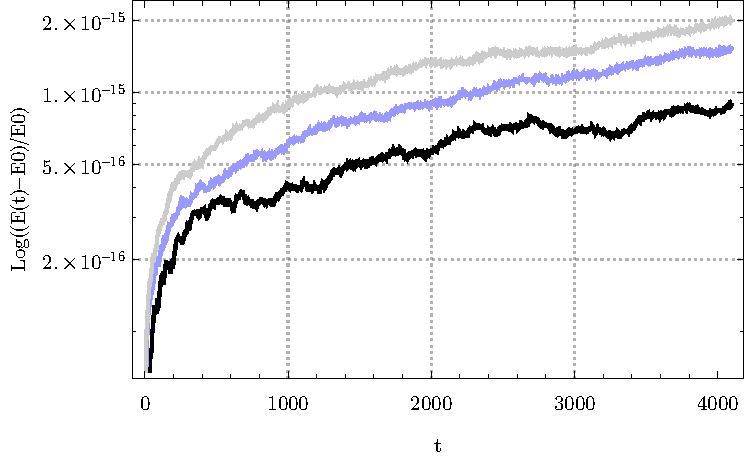
\includegraphics[width=.500\textwidth]{plot3a}
}
\subfloat[Non chaotic: global error.]{
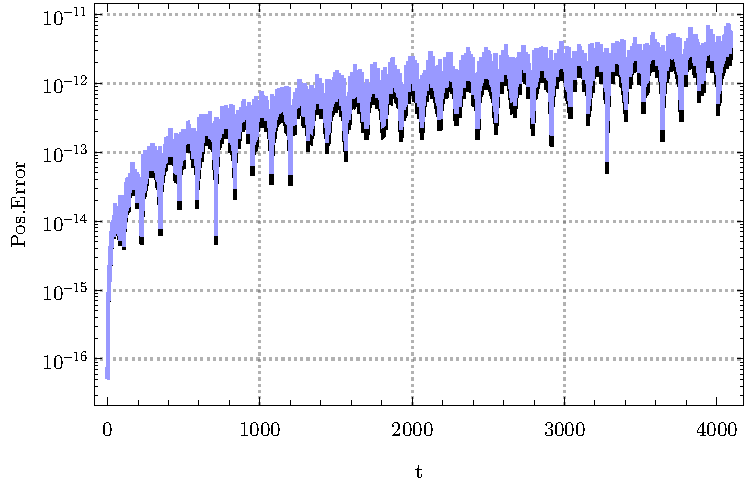
\includegraphics[width=.500\textwidth]{plot3b}
}
\vskip\baselineskip
\subfloat[Chaotic: energy error.]{
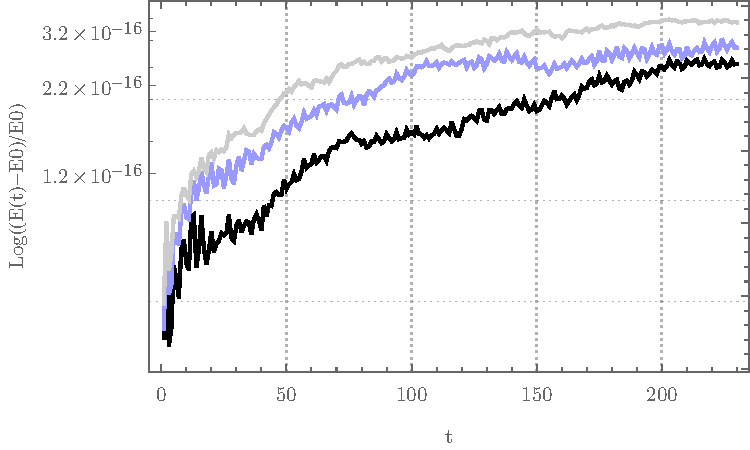
\includegraphics[width=.500\textwidth]{plot3c}
}
\subfloat[Chaotic: global error.]{
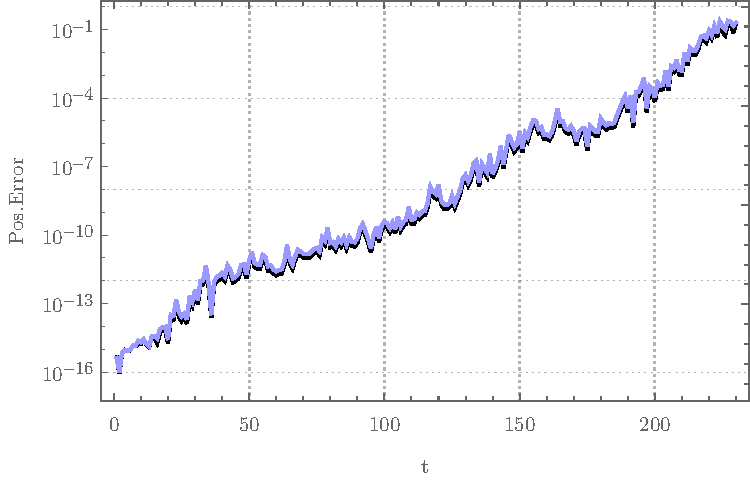
\includegraphics[width=.500\textwidth]{plot3d}
}
\caption[Pendulu-bikoitza: energiaren errorearen eta errore globalaren eboluzioa.]{\small We show Non-Chaotic case (a,b) and Chaotic case (c,d). Left figure mean energy error evolution $\bar{\triangle E_i}$ and right figure mean Global error evolution $\bar{Ge_i}$ of the 100 integrations for \textit {Ideal Integrator} (black) , \textit {Double prec} (blue) and \textit {Classic Implementation} (gray).}
\label{fig:plot3}
\end{figure}

\subsection*{Brouwer-legea.}


\begin{figure}[h]
\centering
\subfloat[Non-Chaotic: Ideal.]{
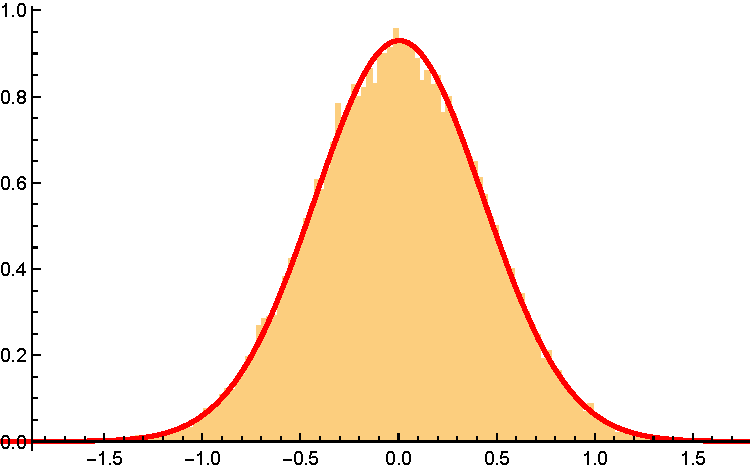
\includegraphics[width=.450\textwidth]{brouwer4a}
}
\subfloat[Non-Chaotic: rdigits=0.]{
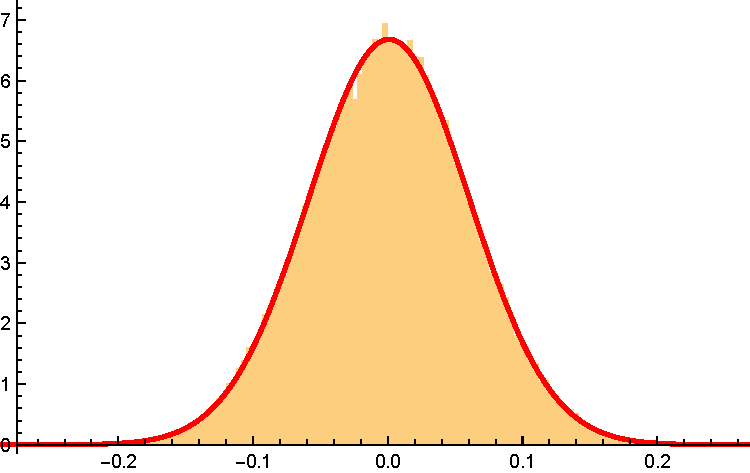
\includegraphics[width=.450\textwidth]{brouwer4b}
}
\vskip\baselineskip
\subfloat[Chaotic: Ideal.]{
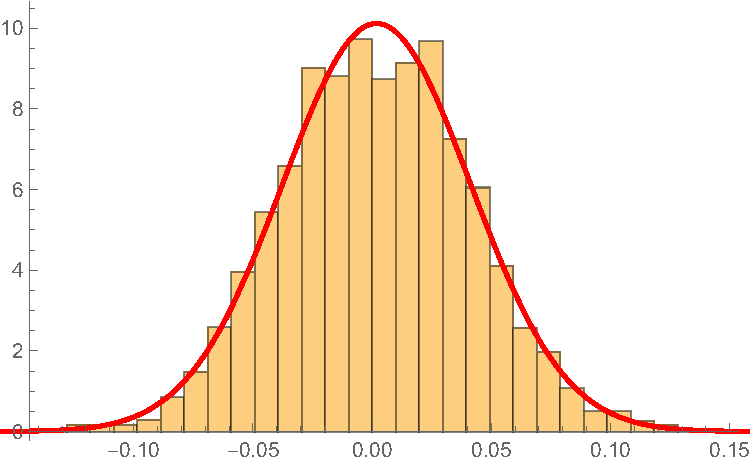
\includegraphics[width=.450\textwidth]{brouwer4c}
}
\subfloat[Chaotic: rdigits=0.]{
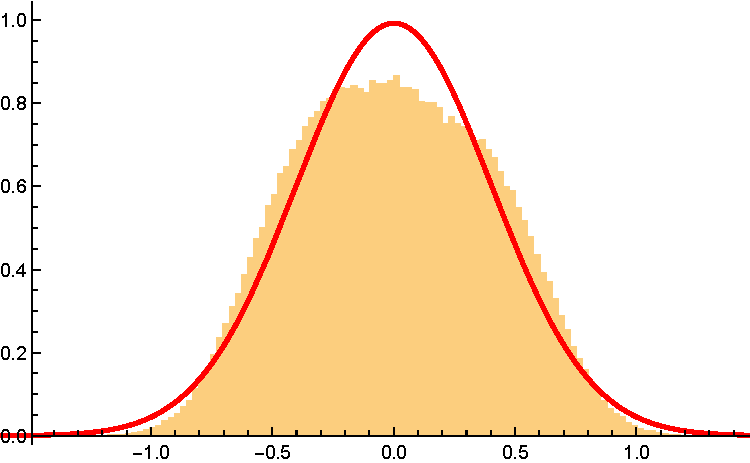
\includegraphics[width=.450\textwidth]{brouwer4d}
}
\caption{ \small Histogram of energy errors for Non-Chaotic case (a,b) and for Chaotic case (c,d).}
\label{fig:brouwer103}
\end{figure}

\subsection*{Biribiltze erroreaen estimazioa.}


\begin{figure}[h]
\centering
\subfloat[Non Chaotic: estimation]{
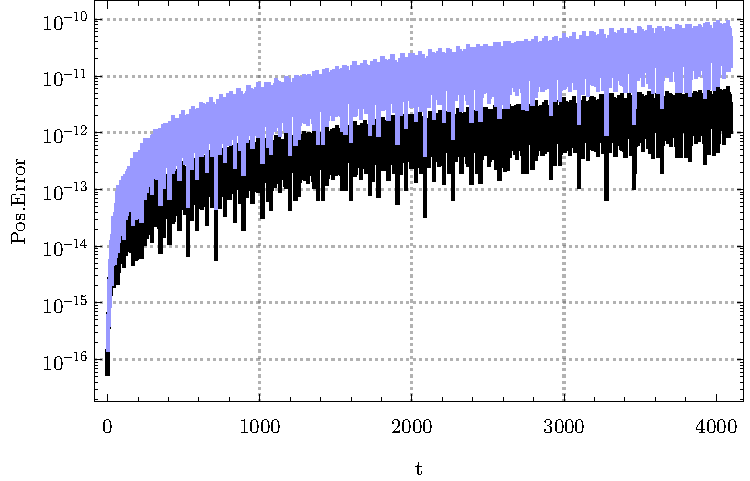
\includegraphics[width=.500\textwidth]{plot5a}
}
\subfloat[Non Chaotic: quality of estimation]{
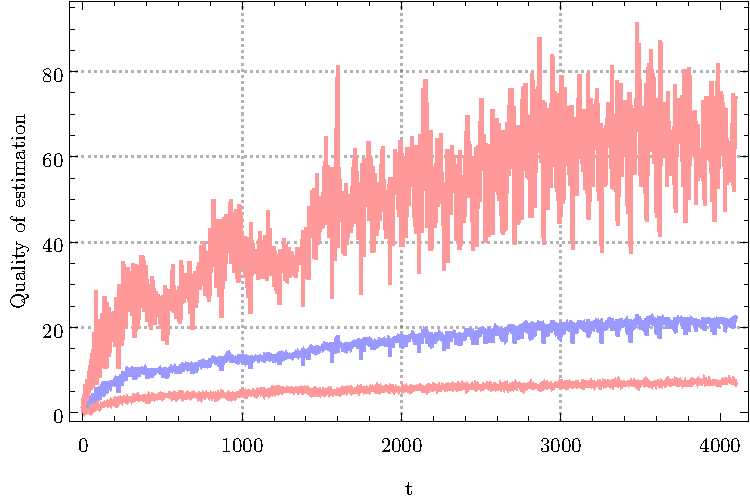
\includegraphics[width=.500\textwidth]{plot5b} 
}
\vskip\baselineskip
\subfloat[Chaotic: estimation]{
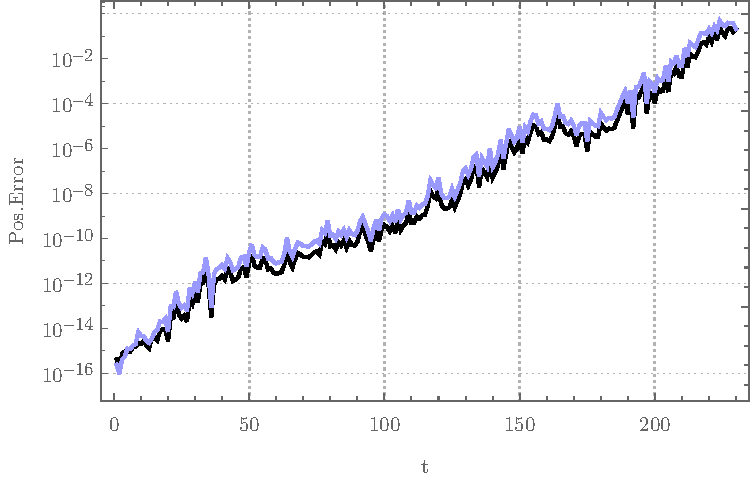
\includegraphics[width=.500\textwidth]{plot5c} 
}
\subfloat[Chaotic: quality of estimation]{
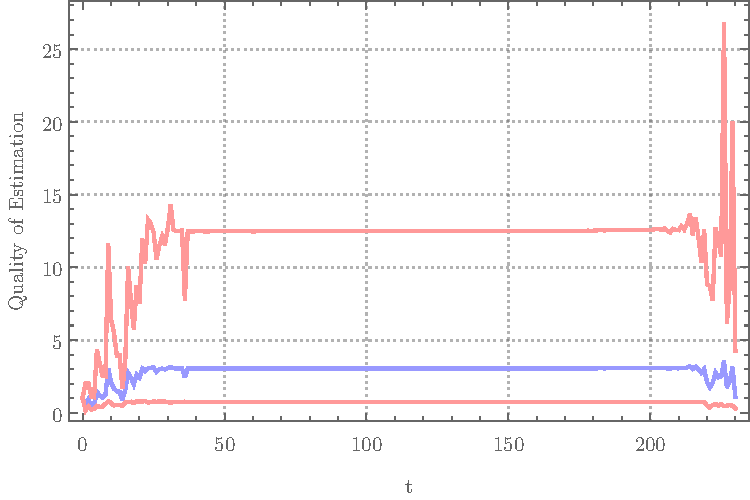
\includegraphics[width=.500\textwidth]{plot5d}
}

\caption[Pendulu-bikoitza: biribiltze errorearen estimazio.]{\small Estimation round-off error. We compare evolution of our estimation error (blue) with evolution of global error (black). Estimation Quality. We show mean (blue) and  standard deviation (red) of the quality according our definition of (\ref{eq:eq_Qi}).}
\label{fig:plotest}
\end{figure}

\subsection{N-Body problema.}


\begin{figure}[h]
\centering
\subfloat[Energy error.]{
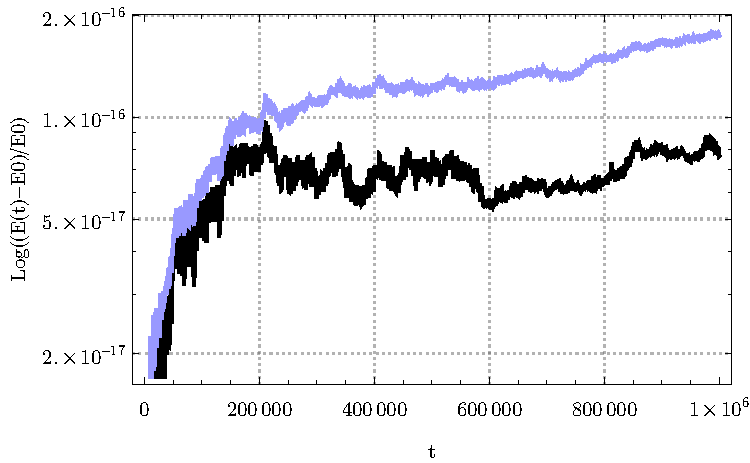
\includegraphics[width=.500\textwidth]{plot6a}
}
\subfloat[Global error.]{
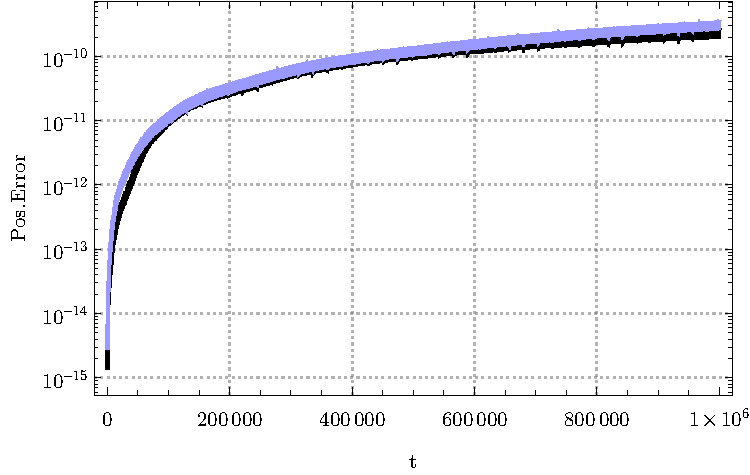
\includegraphics[width=.500\textwidth]{plot6b}
}
\caption[N-Body: energiaren errorearen eta errore globalaren eboluzioa.]{\small N-body: left figure mean energy error evolution $\bar{\triangle E_i}$ and right figure mean Global error evolution $\bar{Ge_i}$ of the 100 integrations for Ideal Integrator (black) and Double prec(blue).}
\label{fig:nbody1}
\end{figure}

\begin{figure}[h]
\centering
\subfloat[Estimation.]{
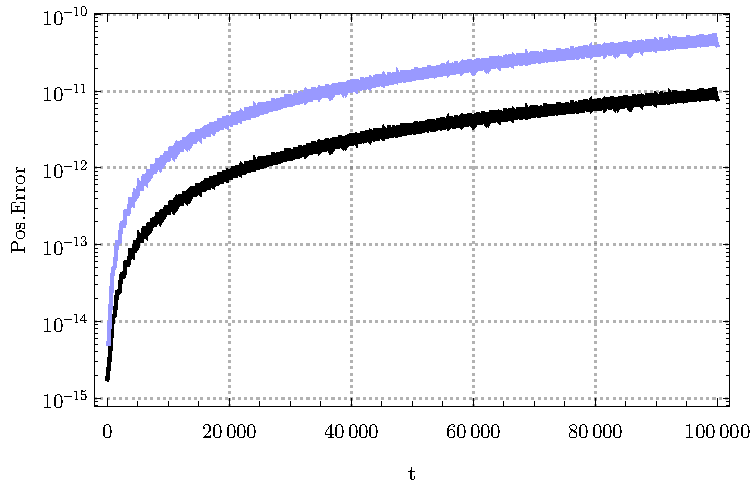
\includegraphics[width=.500\textwidth]{plot7a}
}
\subfloat[Quatlity.]{
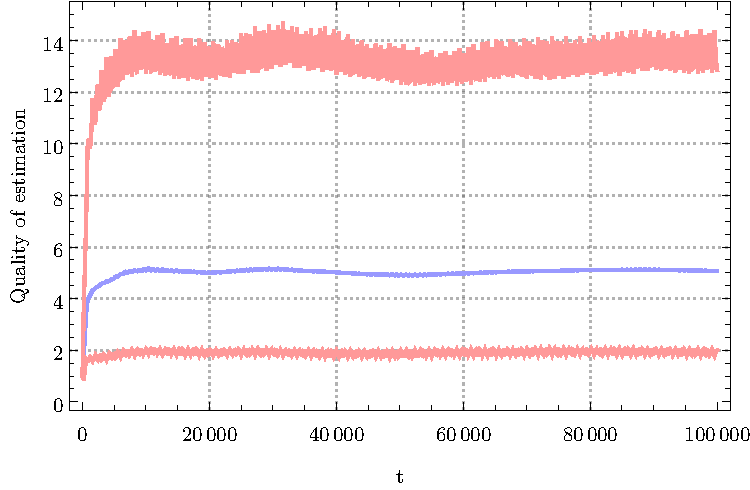
\includegraphics[width=.500\textwidth]{plot7b}
}
\caption[N-Body: birbiltze errorearen estimazioa.]{\small Left estimation round-off error, we compare evolution of our estimation error (blue) with evolution of global error (black). Right estimation Quality ,we show mean (blue) and  standard deviation (red) of the quality according our definition of (\ref{eq:eq_Qi}). We use rdigits1=0 and rdigits2=3.}
\label{fig:nbody2}
\end{figure}


